\documentclass{nime-alternate} % Uncomment when publishing final version
% Uncomment only one of the ones below
\usepackage{anonymize} 		   %Uncomment this line to publish
% \usepackage[blind]{anonymize}%Uncomment this line for blind review
\usepackage[utf8]{inputenc}

\usepackage{float}
\usepackage{natbib}
\usepackage{graphicx}
\usepackage{todonotes}
\usepackage{etoolbox}
\usepackage[inline]{enumitem}
\begin{document}

% --- Author Metadata here. See Template---
\conferenceinfo{NIME'20,}{July 21-25, 2020, Royal Birmingham Conservatoire, ~~~~~~~~~~~~ Birmingham City University, Birmingham, United Kingdom.}
\title{SSS}

\label{key}
\numberofauthors{2} 
\author{
\alignauthor
\anonymize{Amir Salimi}\\
       \affaddr{\anonymize{Department of Computing Science}}\\
       \affaddr{\anonymize{University of Alberta}}\\
       \affaddr{\anonymize{Edmonton,AB,Alberta}}\\
       \email{\anonymize{asalimi@ualberta.ca}}
\alignauthor
\anonymize{Abram Hindle}\\
       \affaddr{\anonymize{Department of Computing Science}}\\
       \affaddr{\anonymize{University of Alberta}}\\
       \affaddr{\anonymize{Edmonton,AB,Alberta}}\\
       \email{\anonymize{abram.hindle@ualberta.ca}}
}

\maketitle

\begin{abstract}
With the generation of novel, high quality, one shot percussive sounds as our end goal, we implemented a set of modular software components utilized to form a pipeline for guided generation of sounds. The most crucial of these components are a "virtual ear" capable of evaluating a sounds proximity to different drum types and an efficient, tractable "virtual synthesizer" with a rich set of parameters and DSP methods capable of generating a wide range of sounds.\\ 
We aimed to design our software such that we can utilize our components in various experimental ways; hence, in order to established an adequate level of confidence in our components, we discuss the implementation, limitations, and evaluations of the "virtual synthesizer" and "virtual ear". Next, we present our findings and assessments in regards to the three different methodologies utilized for the generative process of percussive sounds:  \begin {enumerate*} [label=(\roman*)]
\item random generation \item multivariate distribution sampling and \item evolutionary search.\\
\end {enumerate*} 
Additionally, as we observed a general lack of copyright-free percussive sample-packs as well as a lack of unified approach for obtaining such a data-set by fellow researchers \cite{aouameur2019neural,ramires2019timbfeat}, we aim to ameliorate the issue by presenting a copyright free sample-pack of categorized percussion sounds. Furthermore, we have included in our project source code \footnote{\url{https://github.com/imilas/Synths_Stacks_Search}} a set of scripts to further expand the sample pack via royalty free sources. 
\keywords{drum, percussion, synthesis, MIR, ML, genetic, search}
\end{abstract}
% See template for CCS classification. 
\ccsdesc[500]{Applied computing~Sound and music computing}
\ccsdesc[500]{Information systems~Music retrieval}
\printccsdesc

\section{Introduction}
\subsection{Background and Motivation}
The rise of Digital Audio Workstations (DAW) \cite{leider2004digital} and Virtual Studio Technology (VST) based plug-ins \cite{tanev2013virtual} have rapidly transformed the sonic and material landscape of music production in the recent years. Coupled with this rise in popularity is a vast array of commercial products and services dedicated to satiating the need of amateur and professional music producers for unique sounds; most commonly via audio samples: one-shot drum samples, long sustained notes (commonly refered to as pads or textures), percussive or melodic loops etc. Two notable examples of these commercial services are \textit{loopmasters}\footnote{loopmasters.com} and \textit{splice.com}\footnote{splice.com}. Furthermore VST plug-ins can emulate complex audio synthesizers and effects, which some producers may find daunting or time consuming to work with from scratch. In many cases, VST plug-in vendors or unaffiliated enthusiasts sell additional presets for these plugins, targeted towards producers who do not have the time or interest in creating their own. Once a preset is loaded in a VST plug-in, the GUI of the plug-in is updated. Users may modify any loaded preset until their desired sound is observed.\\
Our work is motivated by the idea of finding new, convenient methods for the expansion of a music producer's library of sounds. Primarily with generation of novel, one-shot audio samples but also with automated search and creation of presets for virtual synthesizers that a producer might find  interesting. Using the generation of short, percussive audio samples as a starting point, this project is a proof of concept for promising avenues towards our motivational goal.\\

\subsection{Methodology}
Towards our goal of generating original audio, we found the proper implementation of 2 major components to be crucial:
\begin{itemize}
    \item \textit{Virtual Synthesizer}:A flexible, deterministic, and tractable generator which can create audio. The core of our implementation made use of pippi, \footnote{https://github.com/luvsound/pippi} a fast, offline focused python DSP library with a C backend. We additionally used the scipy \cite{jones2001scipy} library a few audio effects that we found lacking in pippi. 
    \item \textit{Virtual Ear}: An ear that returns an evaluation of an audio sample; estimating the effectiveness of an audio sample's fulfillment of a producers requirements. The implementation and training of the ear guides the generation process towards a desired path.\\
\end{itemize}
Following the Unix Philosophy \cite{gancarz2003linux}, our components are designed with modularity and parallelizability in mind. This allows each component to be debugged, modified and improved without requiring modifications in other components; additionally, increasing the scalability and speed of experiments.
Section \ref{impl} contains further discussion of the components as well as the code that glues the project together can be found in .\\ 
While the main focus of this project is the generation of novel percussive sounds, our methodology indicates promising results with regards to creation of new presets for any virtual synth without the need for a-priori knowledge of the functions of its parameters (i.e the effect of parameter modulation on the sonic output). We also demonstrate the viability of a few lesser explored avenues for the purposes of audio synthesis and Music Information Retrieval (MIR), notably:
\begin{enumerate}[label=\roman*]
\item Heuristic search methods for the creation of new presets for virtual synthesizers. More concretely, we observed that given a virtual ear which could reliably score pieces of audio based on its resemblance to a desired category (e.g:kicks,snares,piano), we were able to rapidly search the parameters of a virtual synthesizer and create numerous parameter-sets (i.e presets) which resemble our desired category of sounds.
\item The viability of virtual synthesizers based on Digital Signal Processing (DSP) methods for fast, unsupervised creation of novel audio, discussed in more detail in section \ref{related}. \\
\end{enumerate}

\subsection{Related Work and Contradistinctions}
\label{related}
Numerous deep, neural network models have been proposed and utilized for the purpose of signal generation in recent years. WaveGans and WaveNet have been subject to significant improvements and experiments since their proposal \cite{nsynth2017} and recently, Variational AutoEncoders (VAE's) have been utilized for generation of short percussive samples \cite{aouameur2019neural,ramires2019timbfeat}. In this work however, we opt to use digital signal processing methods to create a virtual synthesizer for the generation of audio signals, as it provides several unique advantages:
\begin{enumerate}[label=\roman*]
  \item Fast, offline rendering of audio with no relience on GPU, currently not possible with state of the art models such as parallel WaveGan \cite{yamamoto2019parallel} and parallell WaveNet \cite{oord2017parallel}. 
  \item Rendering at high sampling rates with little performance issues: Commonly, likely to speed up performance, the standard sampling rate in most audio generation work with neural networks appears to be under 24 khz. However, a significant number of untrained human ears can detect a change in quality of audio between sampling rates of 192 khz and the industry standard of 44.1 khz \cite{reiss2016meta}, with a dramatic increase in quality detection after training. Therefore we can safely assume that most producers would prefer their audio samples have sampling rates of 44.1 khz or higher. \cite{yamamoto2019parallel,oord2017parallel,aouameur2019neural,ramires2019timbfeat}
  \item Neural networks are often viewed as unexplainable black box solutions. Some models such as VAE's can learn an underlying latent space of parameters and capture the "essence" of the different labels in a dataset. However, these spaces are learned in an unsupervised manner and must be manually analysed, perhaps extensively, before they can be understood \cite{esling2018generative}. The use of a virtual synthesizer for audio generation makes our parameters readily understandable and easily modifiable. 
\end{enumerate}

\section{Implementation}
\label{impl}
\subsection{Design}
 
\begin{figure}[H]
\centering
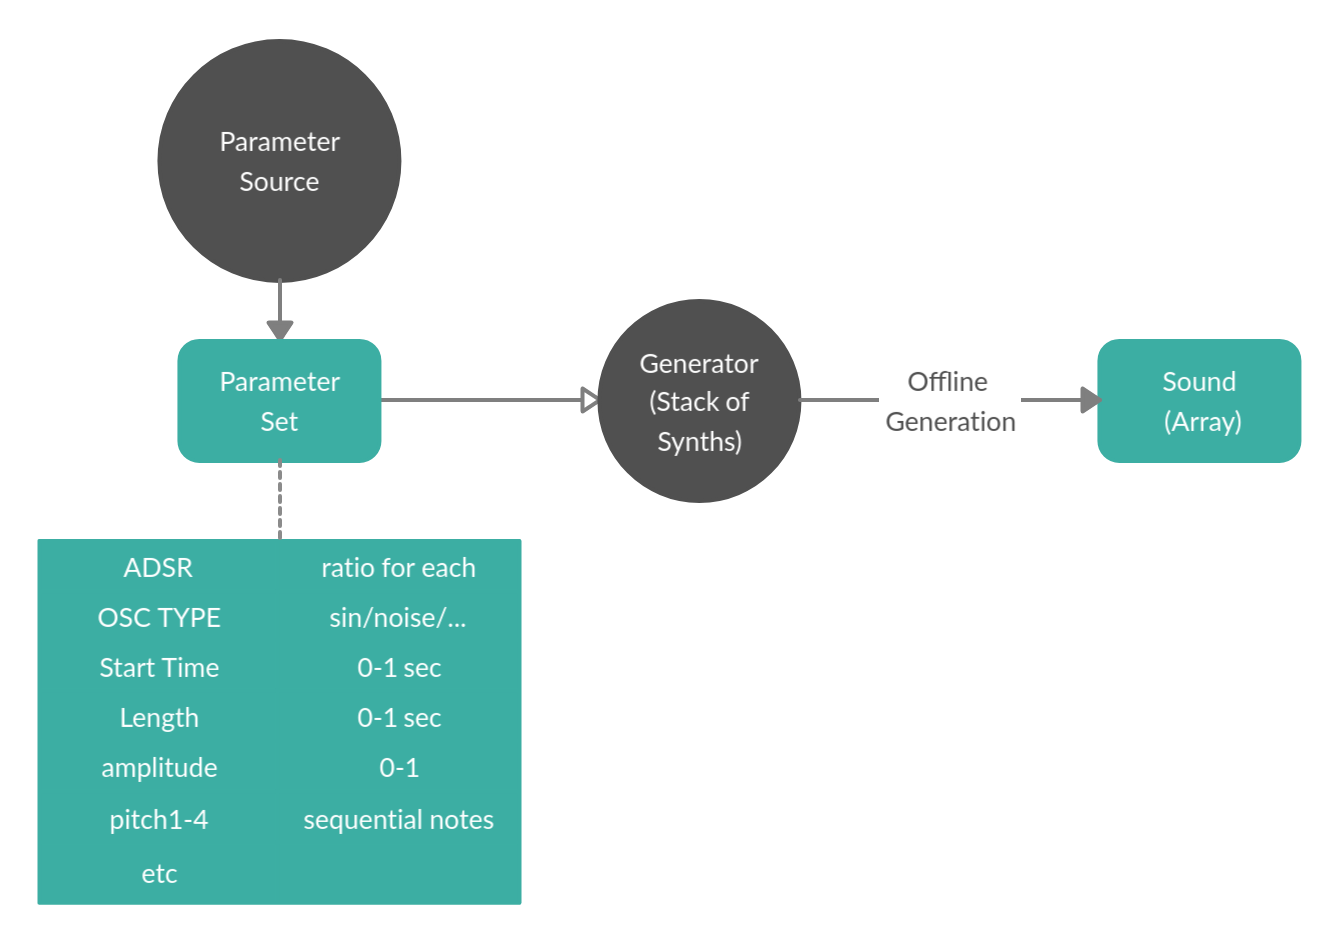
\includegraphics[width=0.9\textwidth]{images/SSS_gen.png}
\caption{Generation Pipeline}
\label{fig:SSS generator}
\end{figure}

\subsection{The Generator}
We used the python based Pippi library for our generator implementation\footnote{https://github.com/luvsound/pippi}. This library uses a C back-end and focuses on fast offline generation. We define a Synth as the smallest unit of sound generation. A single Synth can be fairly expressive on its own, but we also allow a combination of Synths, which we call a Synth Stack. Each Synth takes in multiple parameters (parameter-set) and generates a sound. If the stack size is larger than 1, the combination of these individual parameter-sets is treated as the parameter-set for the stack. 

\subsection{The Ear}
The most challenging and important component of the project; the ear can be any method of evaluating a piece of audio. The most basic representation of a piece of digital audio is via list of numbers and a sampling-rate. For simplicity, we fix the sampling rate to 41,000 per second across all components of this project. An array representation of audio is the representation of the audio within the time domain. More commonly, the frequency domain is used for MIR tasks.
\begin{figure}[H]
\centering
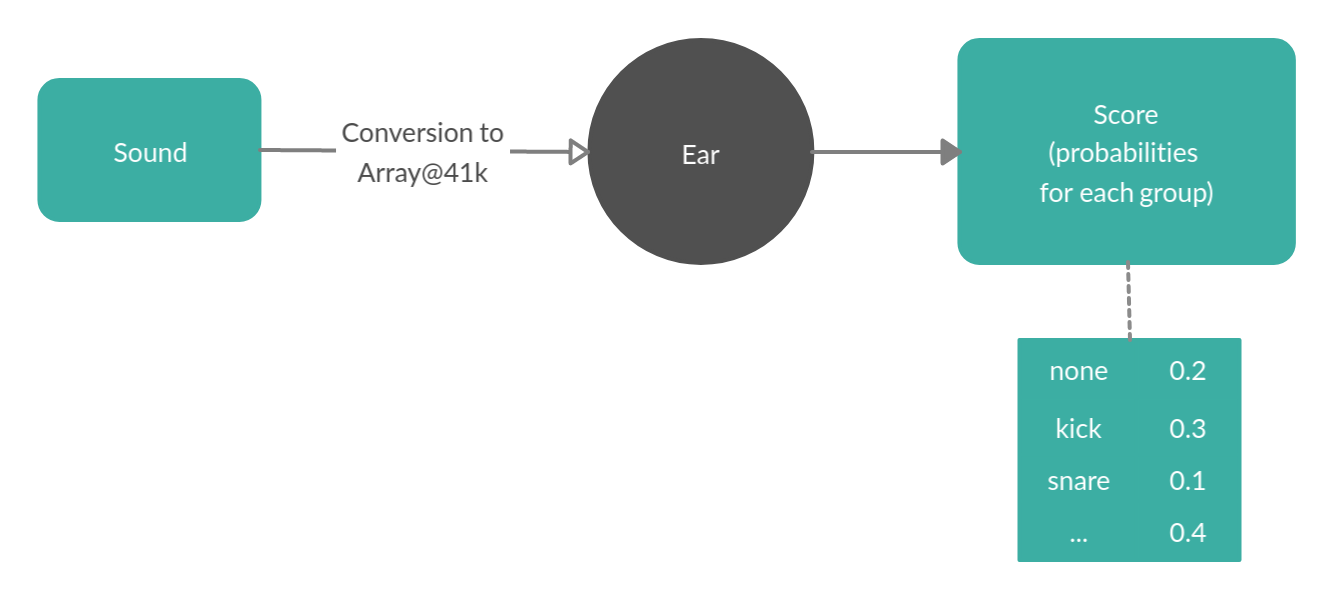
\includegraphics[width=\textwidth]{images/SSS_ear.png}
\caption{Evaluation Using the Ear}
\label{fig:SSS generator}
\end{figure}

\begin{figure}[h!]
\centering
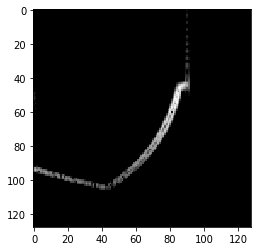
\includegraphics[width=0.5\textwidth]{images/specplot.png}
\caption{Mel-spectrum representation of a randomly generated sample}
\label{fig:SSS generator}
\end{figure}
All we require from the ear is to give us probabilities of an audio sample belonging to various sound (drum and none-drum) categories. It should be self-evident that these probabilities should sum up to 1.\\

We have implemented several methods of feature extraction thus far and successfully separated different drum categories in interesting ways, visualized in the "interactive\_separation\_graph.ipynb" notebook. A common pitfall of most feature extraction methods implemented is that they do not consider the temporal trends within the audio, making them highly susceptible to errors when evaluating audio that should not belong to any of the categories.\\
\todo[inline, color=green!40]{
Sanity Check: If a drum sample is reversed or chopped up, its likelihood of being labeled the same should change.}

There are two interconnected temporal trends to consider: 
\begin{itemize}
    \item Change in amplitude within each frequency bin. Harder to measure and utilize and possibly not as important for our purposes, considering the short length of our samples.
    \item Overall amplitude change within a sample. Closely linked to ADSR. 
\end{itemize}{}

Temporal trends are can be deduced from a spectrum representation of sound (at least visually by a human). A convolution net trained on our drum dataset led to an ear good enough to continue to the next stage of the project. The current model does an adequate job of rejecting junk data and semi-robustly rejects samples with inappropriate wave-shapes.
\begin{figure}[H]
\centering
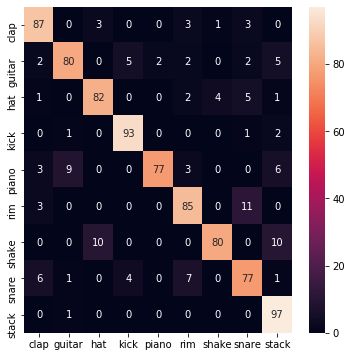
\includegraphics[width=0.8\linewidth]{images/cnn_ear.png}
\caption{CNN ear working well on a test set}
\label{fig:ok ear}
\end{figure}

\subsection{Generator+Ear}
Once we have a generator and an ear, we can quickly generate a large dataset where each data item is a random parameter-set, the ear score of the parameter-set and the corresponding rankings for each category. The rankings are derived from the probability scores. For example, the category with the highest probability will have the rank of 1, second highest would rank 2nd, and the lowest probability will have the rank of n (assuming n categories).\\
Important to highlight is that thus far we have only used 1 Synth to generate our sounds, but our generator has the capability to use larger Synth Stacks, and the pipelines are written with that possibility in mind.\\
\todo[inline]{A seen in Figure \ref{fig:rank portions}, there is a bias in random generation towards making higher ranking hats and kicks and lower ranking shakers, claps. Is this bias because of Synth structure or a problem with the ear?}
\begin{figure}[h!]
\centering
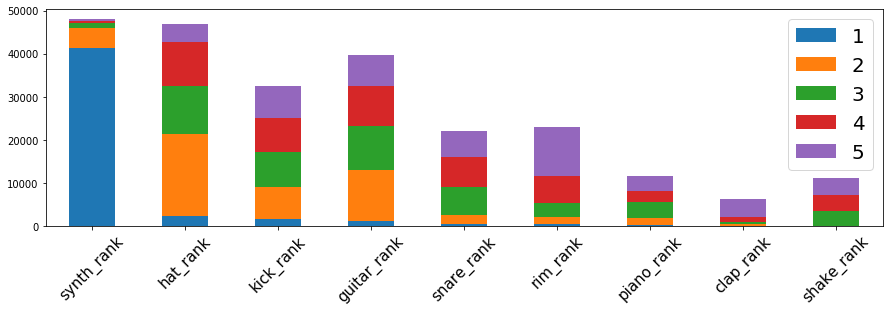
\includegraphics[width=1\linewidth]{images/random_ranks.png}
\caption{Figure showing proportions of categorical ranks for around 50,000 randomly generated sounds. Only showing ranks 1-5. About 90\% received the rank of 1 (blue portion of the bar) for the "synth" category, meaning that the ear correctly gave the highest probability to the sound being from a synth combination. We are interested in the small percentages of random generations that trick the ear due to coincidentally being similar to actual drums (i.e those who received a rank of 1) }
\todo[inline, color=green!30]{When looking for the best sounds of each category, could use ranks 2 and 3 etc. as well, however:
\unexpanded{\unexpanded{
\begin{itemize}
    \item We must figure out how to penalize their parameters
    \item The task requires even more confidence in ear,
    \item Generation is fast enough that we don't need to use ranks higher than 1. We have more than enough data if we don't want to deal with this task.
\end{itemize} 
}}} 


\label{fig:rank portions}
\end{figure}
\section{Novel Generations}
\subsection{Goal}
 Given a category, our aim is to use random generations to guide an algorithm towards novel generation of drums for that category.

\subsection{Guided Generation Attempts}

\subsubsection{Multivariate Normal}
Some success and extremely fast and scalable once the parameter space is calculated. Currently our parameters are array indices mapping to different values for Synth components. This makes the assumption that our discrete parameter space is normally distributed or differentiable in-appropriate and prone to errors. 

\subsubsection{Evolutionary Search}
Implemented evolutionary search using DEAP \citep{DEAP_JMLR2012}. A parameter set is assumed to be an individual with each parameter being its genes. To measure an individuals fitness, we use the formula $fitness=score-rank$. As generations evolve, a Hall-of-Fame list with a fixed size tracks the best individuals to ever live in any given generation, updating itself after each batch of off-springs is evaluated.\\
To ensure diversity of the HOF individuals, the fitness score should also consider some measure of uniqueness. A weighted minkowski distance \footnote{https://docs.scipy.org/doc/scipy/reference/generated/scipy.spatial.distance.minkowski.html} between the genes of an offspring and the HOF individuals may be a good measurement.\\
A generation of $N$ individuals are initialized(randomly or using already existing ranked parameters). To create the offspring generation, each generation goes through mutations and in-place gene crossovers. The new generation consists of the top 80\% of the offspring generation and 20\% new individuals to quicken gene diversity. If the new individuals are coming directly from previously measured high scoring parameter sets, we ensure that they cannot be directly added to HOF without going through mutations and crossovers first. 


\bibliographystyle{abbrv}
    \bibliography{nime-references} 
\end{document}
